\section{Application Characterization}
\label{sec:characterize-app}

  We now turn to measurements of specific popular iOS and Android applications. 
  When users install apps, they grant them Internet access without detailed knowledge of how that access will be used, including {\it how much} data is sent or accessed, {\it what} data is sent,  or {\it with whom} the app communications.
  ``How much'' is important to conserve both bandwidth caps and battery capacity: an app which consumes or produces too much data will waste bandwidth resources, while an app which consumes or produces data too frequently will prevent the device radio from going idle to save power.
  ``With whom'' is important to protect users from excessive tracking -- the more organization's servers an app connects to, the more organizations which are able to track user behavior, location, or other private data.
  Finally, ``what data'' is important because apps may unnecessarily leak personally identifiable information (PII) such as user email address, IMEI, contact information, or other stored data either to the app provider or worse, to any eavesdropper on a public WiFi connection.
  We now report on our findings in all three of these dimensions for the iPhone and Android apps in our study.

\subsection{Bandwidth and Radio Usage}

  {\bf In the Wild.}
    \begin{itemize}
      \item Stats on how much bandwidth each user used; time of day; how frequent...
    \end{itemize}

  {\bf Android Apps.}
    To dig in to the root cause of these usage patterns, we also 

  {\bf iPhone Apps.}

\subsection{Third Party Servers: Ads and Analytic Traffic}

  {\bf In the Wild.}
\begin{figure}
%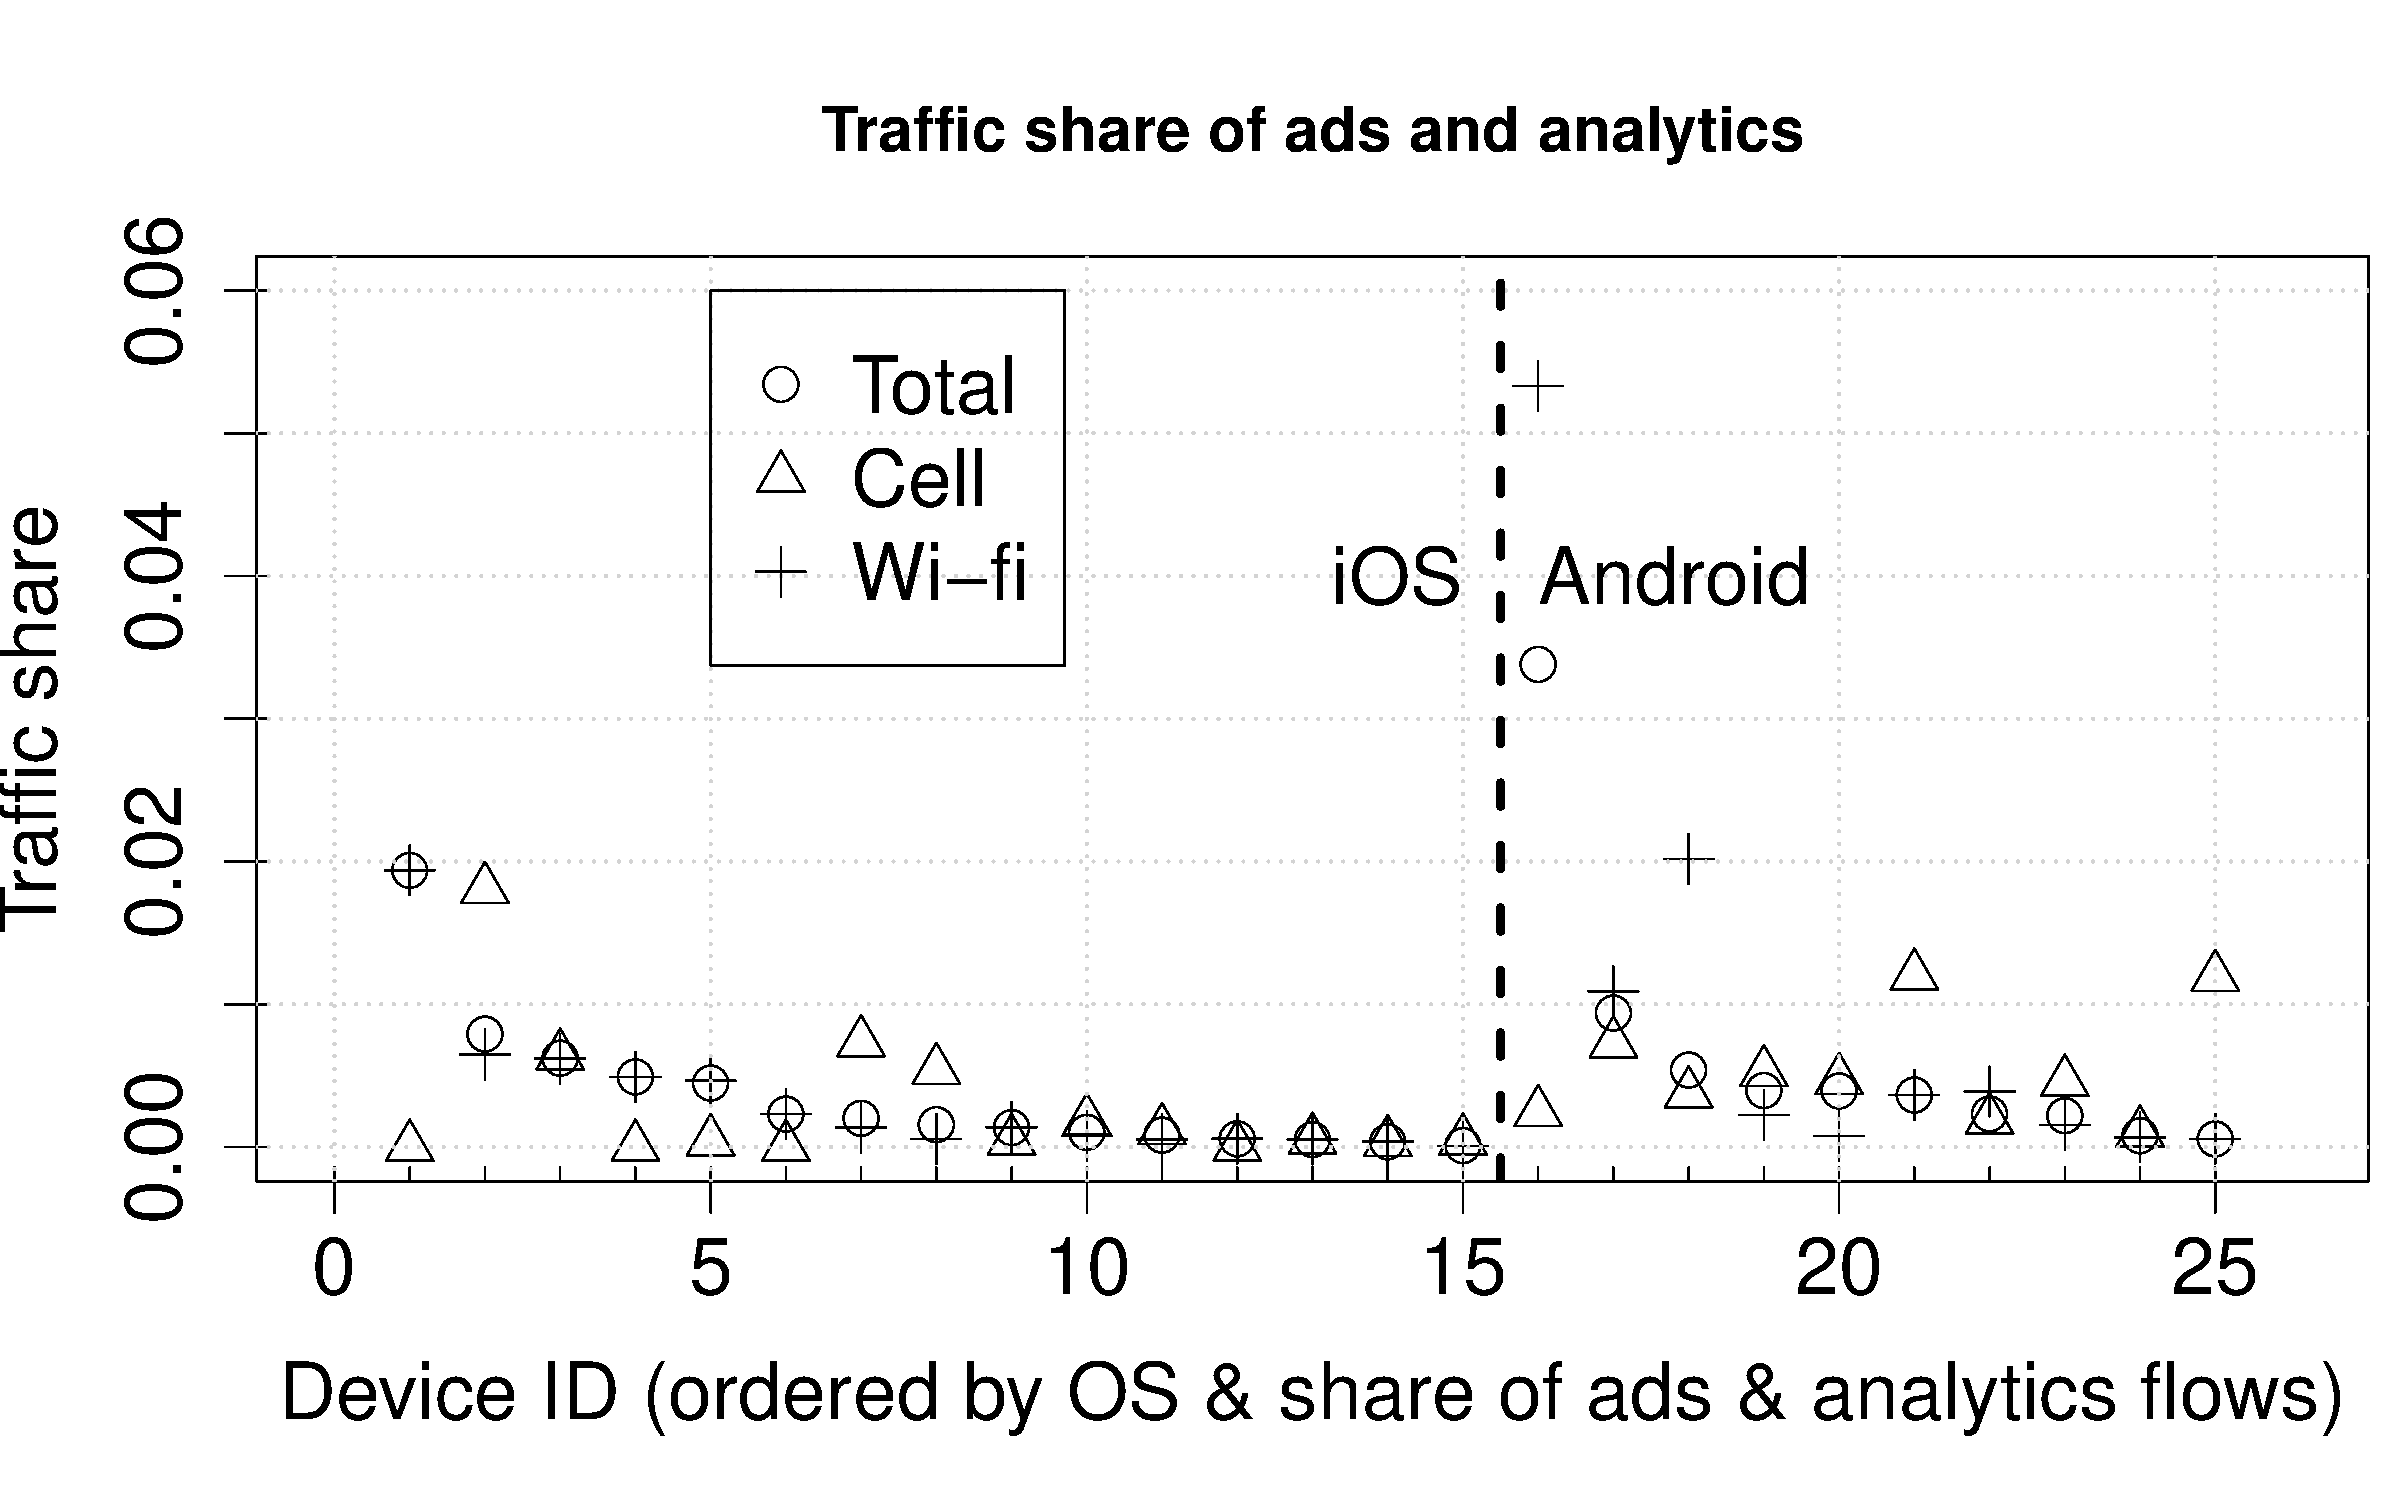
\includegraphics[width=\columnwidth]{plots/ad_share_bytes.pdf}
\caption{Fraction of traffic volume because of Ads and Analytics. \emph{\tbd{Check for id1 and id25}}}
\label{fig:description}
\end{figure}

\begin{figure}
%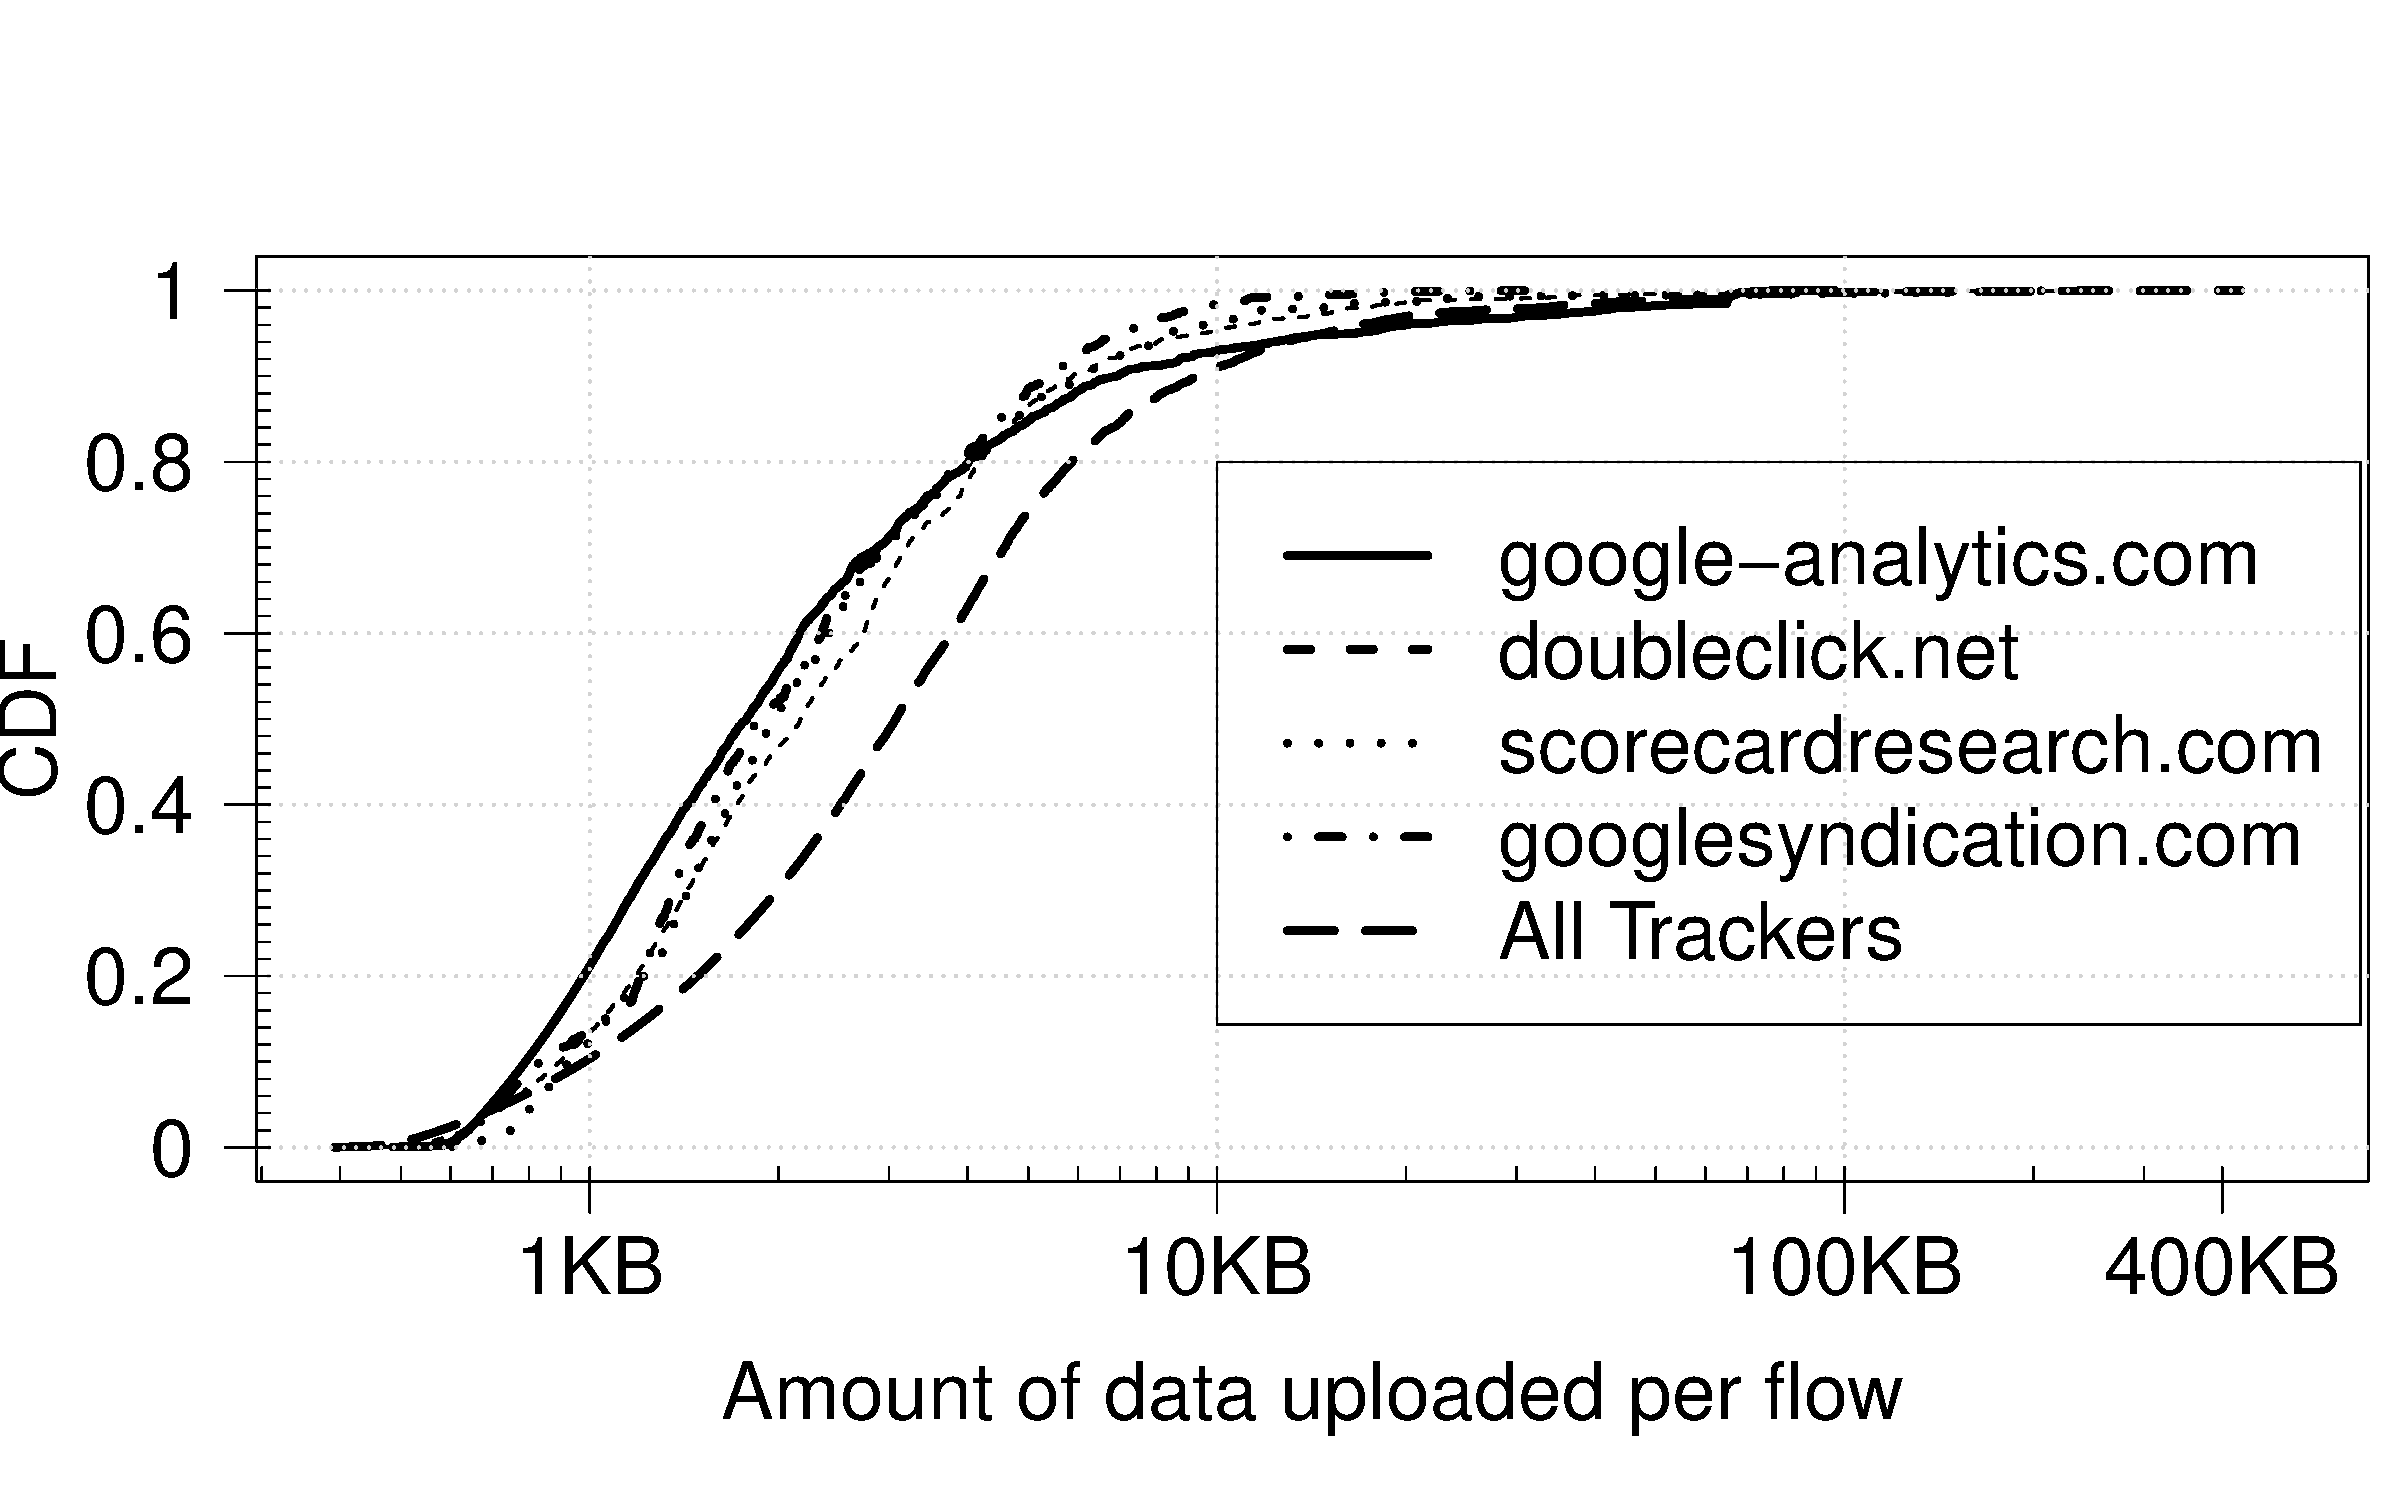
\includegraphics[width=\columnwidth]{plots/distrib_ad_uploads.pdf}
\caption{Distribution of bytes uploaded by ads and analytics sites. \emph{The distribution of bytes uploaded by all ads and analytics sites and the top four ads sites based on traffic volume across all users}.}
\label{fig:description}
\end{figure}

\begin{table}
\begin{small}
\begin{tabular}{|p{0.35\columnwidth}|p{0.1\columnwidth}|p{0.15\columnwidth}|p{0.1\columnwidth}|}
\hline
\multirow{2}{*}{\bf Tracker} & \multicolumn{3}{c|}{\bf Number of devices tracked}\tabularnewline
\cline{2-4}
   &  {\bf Total} & {\bf Android} & {\bf iOS} \tabularnewline
\hline
doubleclick.net & 25 & 11 & 14 \tabularnewline
\hline
google-analytics.com   & 25 & 11 & 14 \tabularnewline
\hline
googlesyndication.com  & 22 & 10 & 12 \tabularnewline
\hline
admob.com  & 21 & 10 & 11 \tabularnewline
\hline
scorecardresearch.com &  21 & 10 & 11 \tabularnewline
\hline
2mdn.net  &  20 & 9 &  11 \tabularnewline
\hline
atdmt.com  & 18 & 9 &  9 \tabularnewline
\hline
imrworldwide.com & 18 &  9 &  9 \tabularnewline
\hline
flurry.com & 17 & 7 &  10 \tabularnewline
\hline
googleadservices.com  & 17 & 8 &  9 \tabularnewline
\hline
\end{tabular}
\end{small}
\caption{The top 10 ads and analytics sites that tracked the devices in our dataset.
\emph{Two trackers, \emph{doubleclick.net} and\emph{google-analytics.com}, were tracking all the 25 devices in our dataset.}}
\label{tab:top_trackers}
\end{table}

  {\bf Android Apps.}

  {\bf iPhone Apps.}


\subsection{Personally Identifiable Information}

  {\bf Android Apps.}

  {\bf iPhone Apps.}

\subsection{Characterize Facebook Applications}

Why Facebook was chosen?

What do we observe ?

What do we see in the User Agent Fields. 


